\documentclass{article}

%\usepackage{graphicx}

%\usepackage{amsmath}

\usepackage{gvv-book}

\usepackage{gvv}

%\usepackage{float}

\usepackage{enumitem}

%\usepackage{tfrupee}

%\title{CBSE}

%\usepackage{romannum}

%\date{september 2024}

\begin{document}

\begin{enumerate}
	\item In \figref{fig:circleABC}, $PQ$ is a tangent at point $C$ to a circle with center $O$. If $AB$ is a diameter and $\angle CAB = 30^{\degree}$, find $\angle PCA$.
	\begin{figure}[H]
          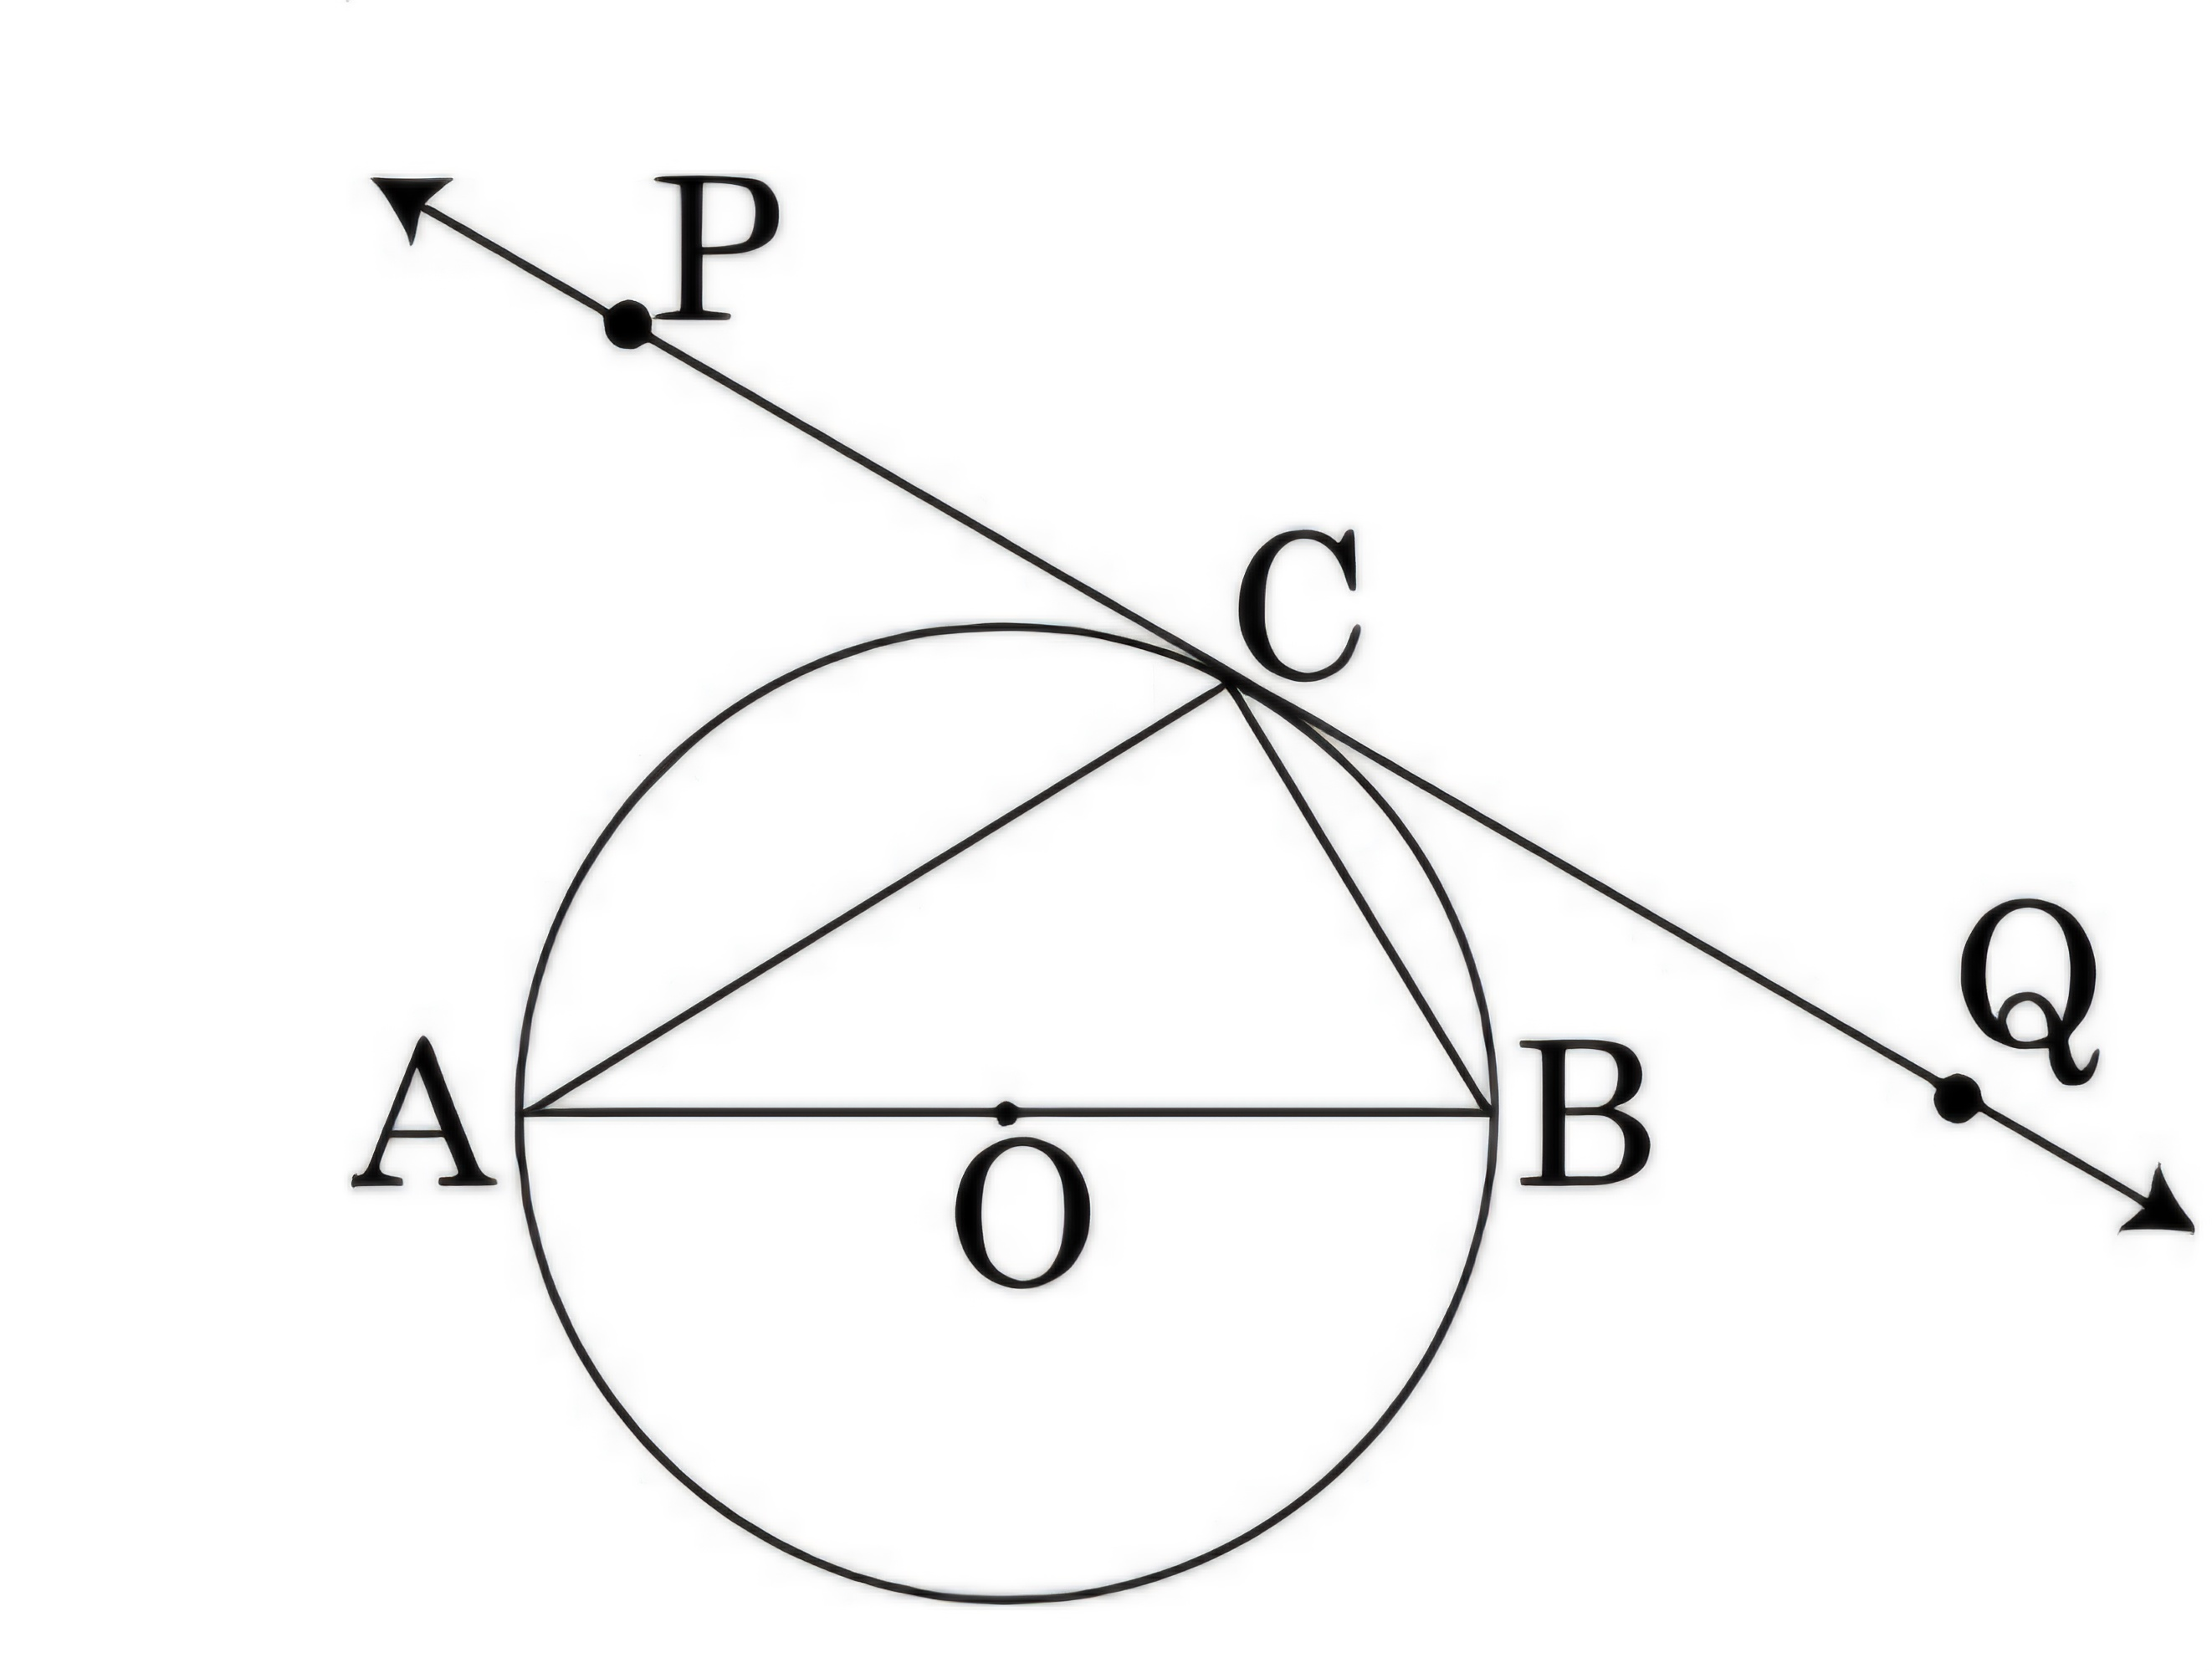
\includegraphics[width=\columnwidth]{./figs/circleABC.jpg}
           \caption{CircleABC}
            \label{fig:circleABC}
         \end{figure}
 
\item If $-5$ is a root of the quadratic equation $2x^2+px-15=0$ and the quadratic equation $p(x^2+x)+k=0$ has equal roots, find the value of $k$.
\item Let $P$ and $Q$ be the points of trisection of the line segment joining the points $A(2, -2)$ and $B(-7,4)$ such that $P$ is nearer to $A$. find the coordinates of $P$ and $Q$.
\item the $4^{th}$ term of an A.P. is zero. Prove that the $25^{th}$ term of the $A.P$ is three times its $11^{th}$ term.
\item In \figref{fig:circle}, $O$ is the centre of a circle such that diameter $AB=13 cm$ and $AC=12 cm$. $BC$ is joined. Find the area of the shaded region. (Take $\pi=3.14$)
 \begin{figure}[H]
   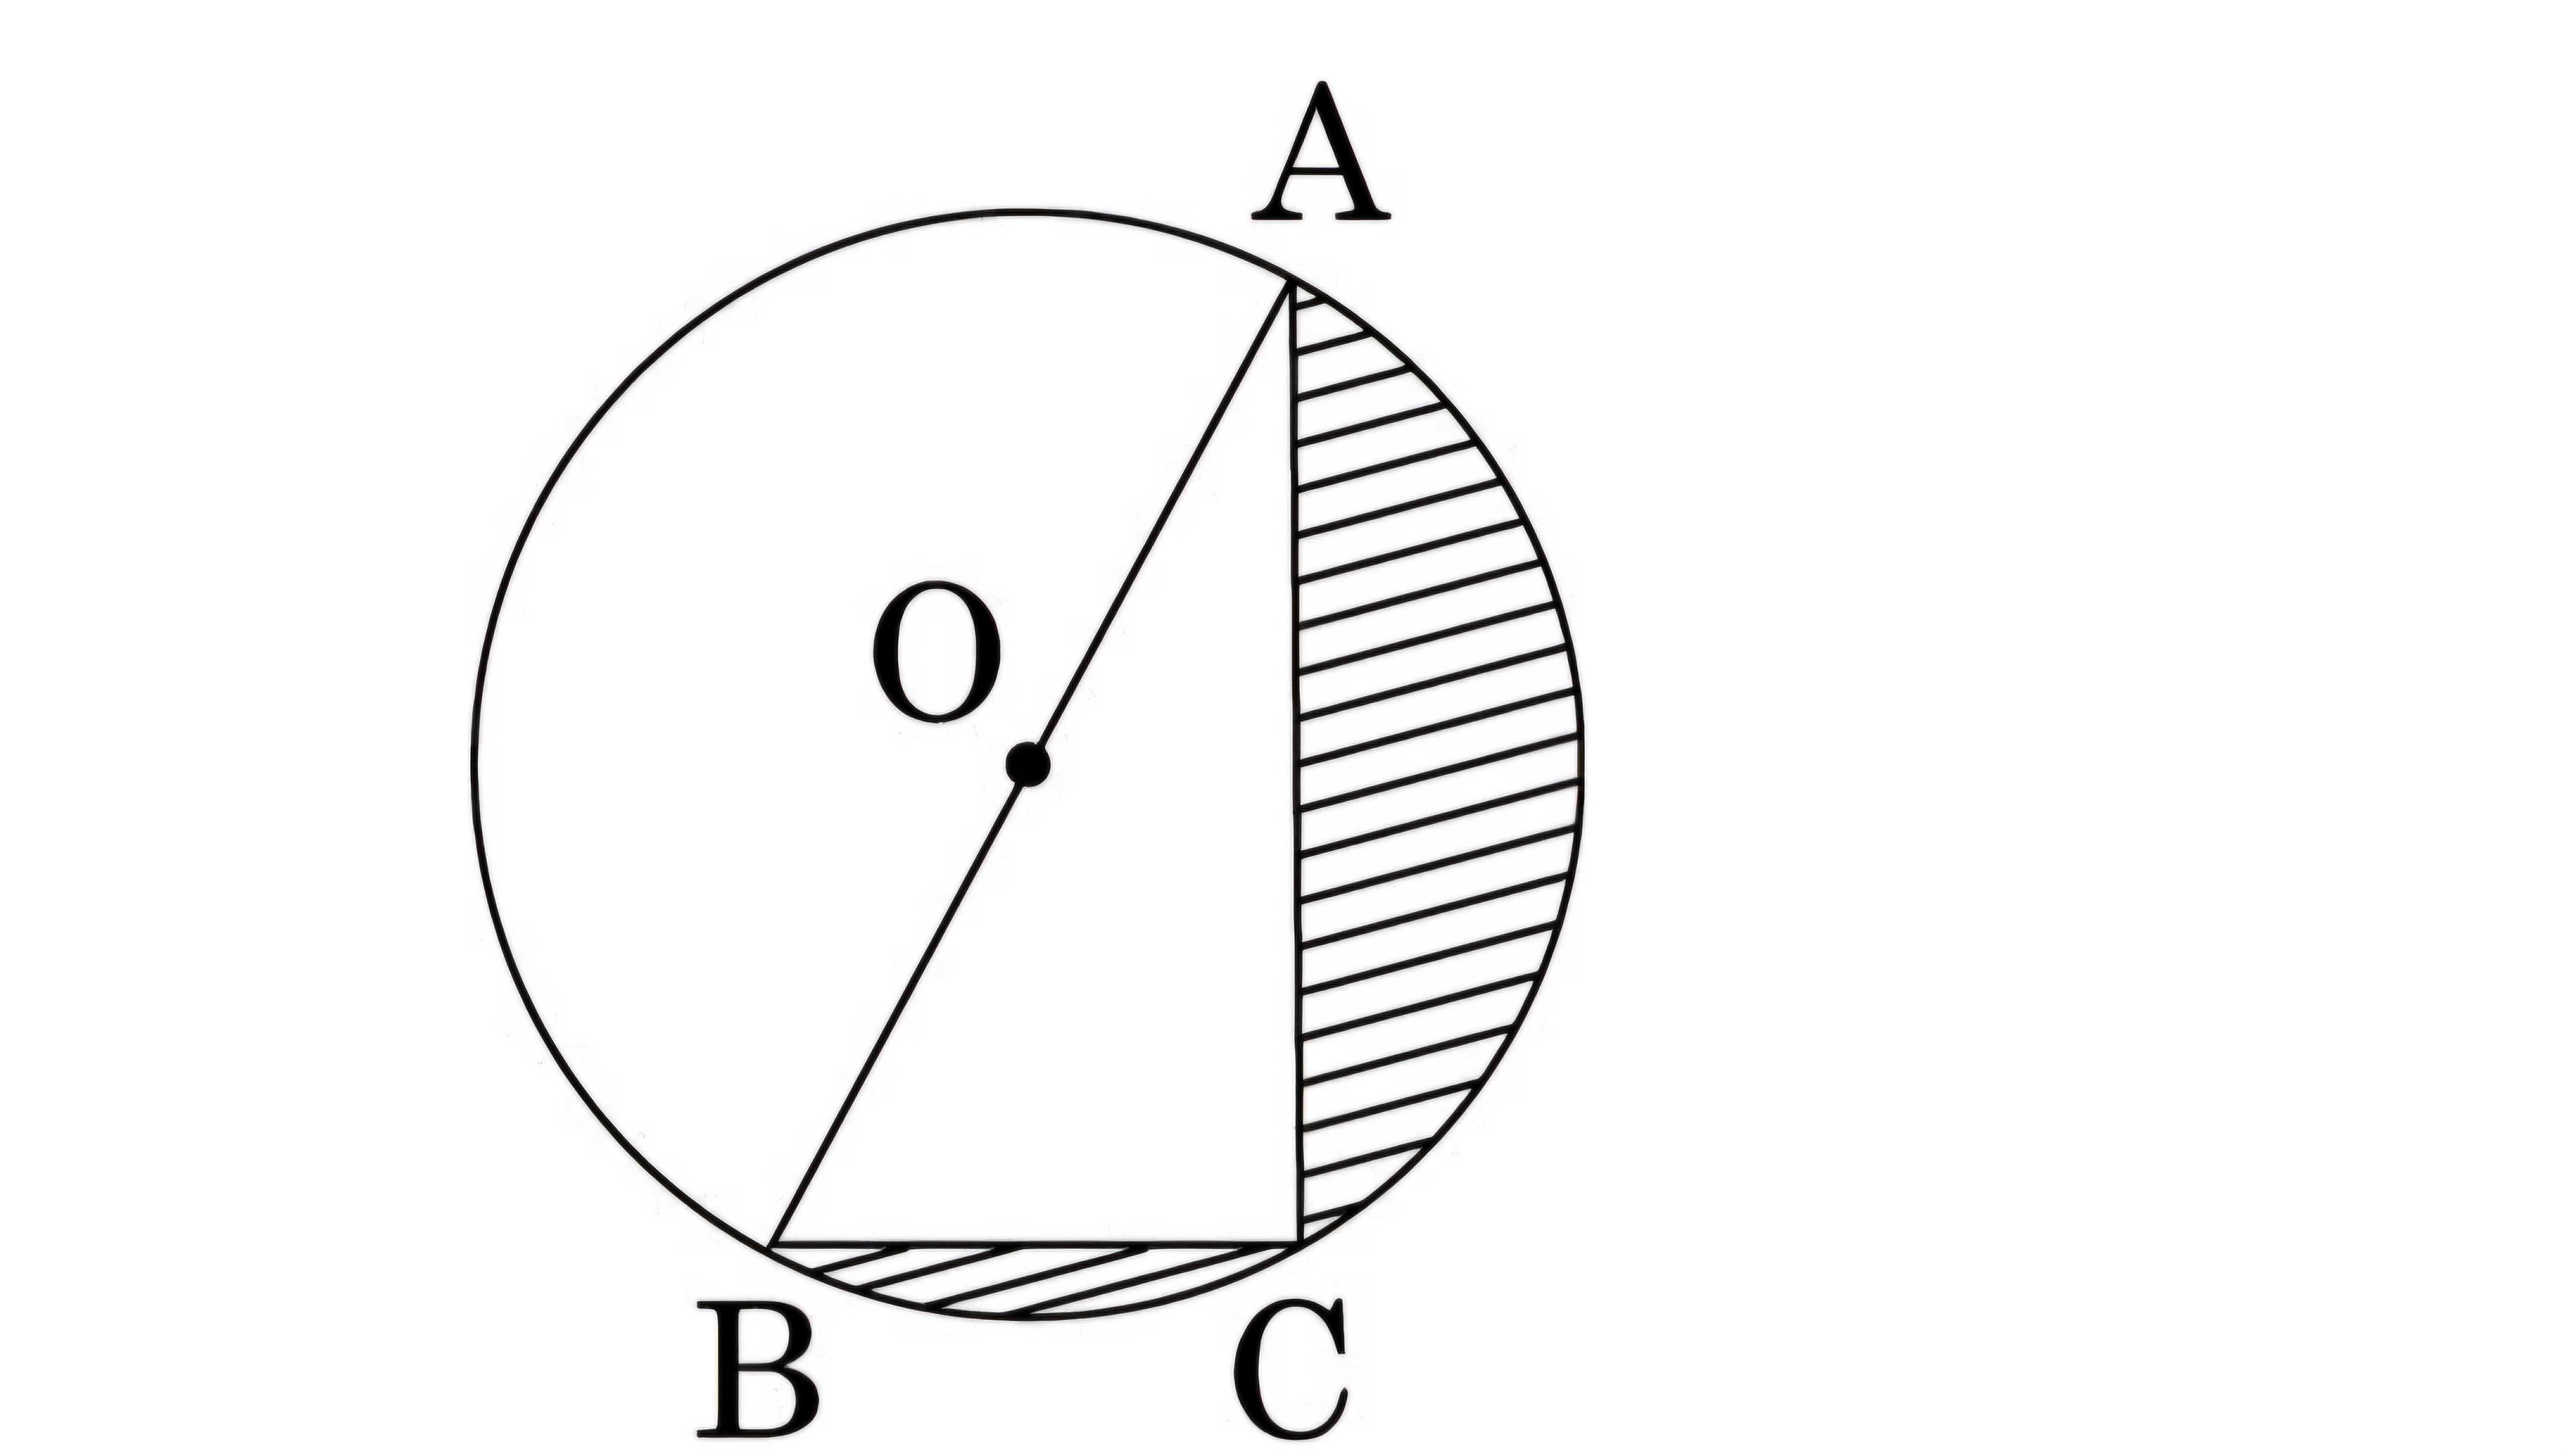
\includegraphics[width=\columnwidth]{./figs/circle.jpg}
    \caption{Circle with centre O}
     \label{fig:circle}
      \end{figure}
\item If the point $P(x, y)$ is equidistant from the points $A(a+b, b-a)$ and $B(a-b, a+b)$. prove that $bx=ay$
\item If the ratio of the sum of first $n$ terms of two 5A.P's is $(7n+1):(4n+27)$, find the ratio of their $m^{th}$ terms.
\item solve for $x$:
	\begin{align}
		\frac{1}{(x-1)(x-2)}+\frac{1}{(x-2)(x-3)}=\frac{2}{3},x \not= 1,2,3 
	\end{align}
\item A man standing on the deck of a ship,which is $10 m$ above water level, observes the angle of elevation of the top of a hill as $60^{\degree}$ and the angle of depression of the base of hill as $30^{\degree}$. Find the distance of the hill from the ship and the height of the hill.
\item Three different coins are tossed together. Find the probability of getting
	      \begin{enumerate}[label=\roman*]
 \item exactly two heads,
							
 \item at least two heads
						
 \item at least two tails.
	      \end{enumerate}
\item prove that the lengths of the tangents drawn from an external point to a circle are equal.				
\item Drawn a circle of radius $4 cm$. Drawn two tangents to the circle inclined at an angle of $60^{\degree}$ to each other.
\item In \figref{fig:twocircle}, two equal circles,with centres $O$ and $O'$, touch each other at $X$.$OO'$ produced meets the circle with centre $O'$ at $A$. $AC$ is tangent to the circle with centre $O$, at the point $C$. $O'D$ os perpendicular to $AC$. Find the value of $\frac{DO'}{CO}$.
  \begin{figure}[H]
   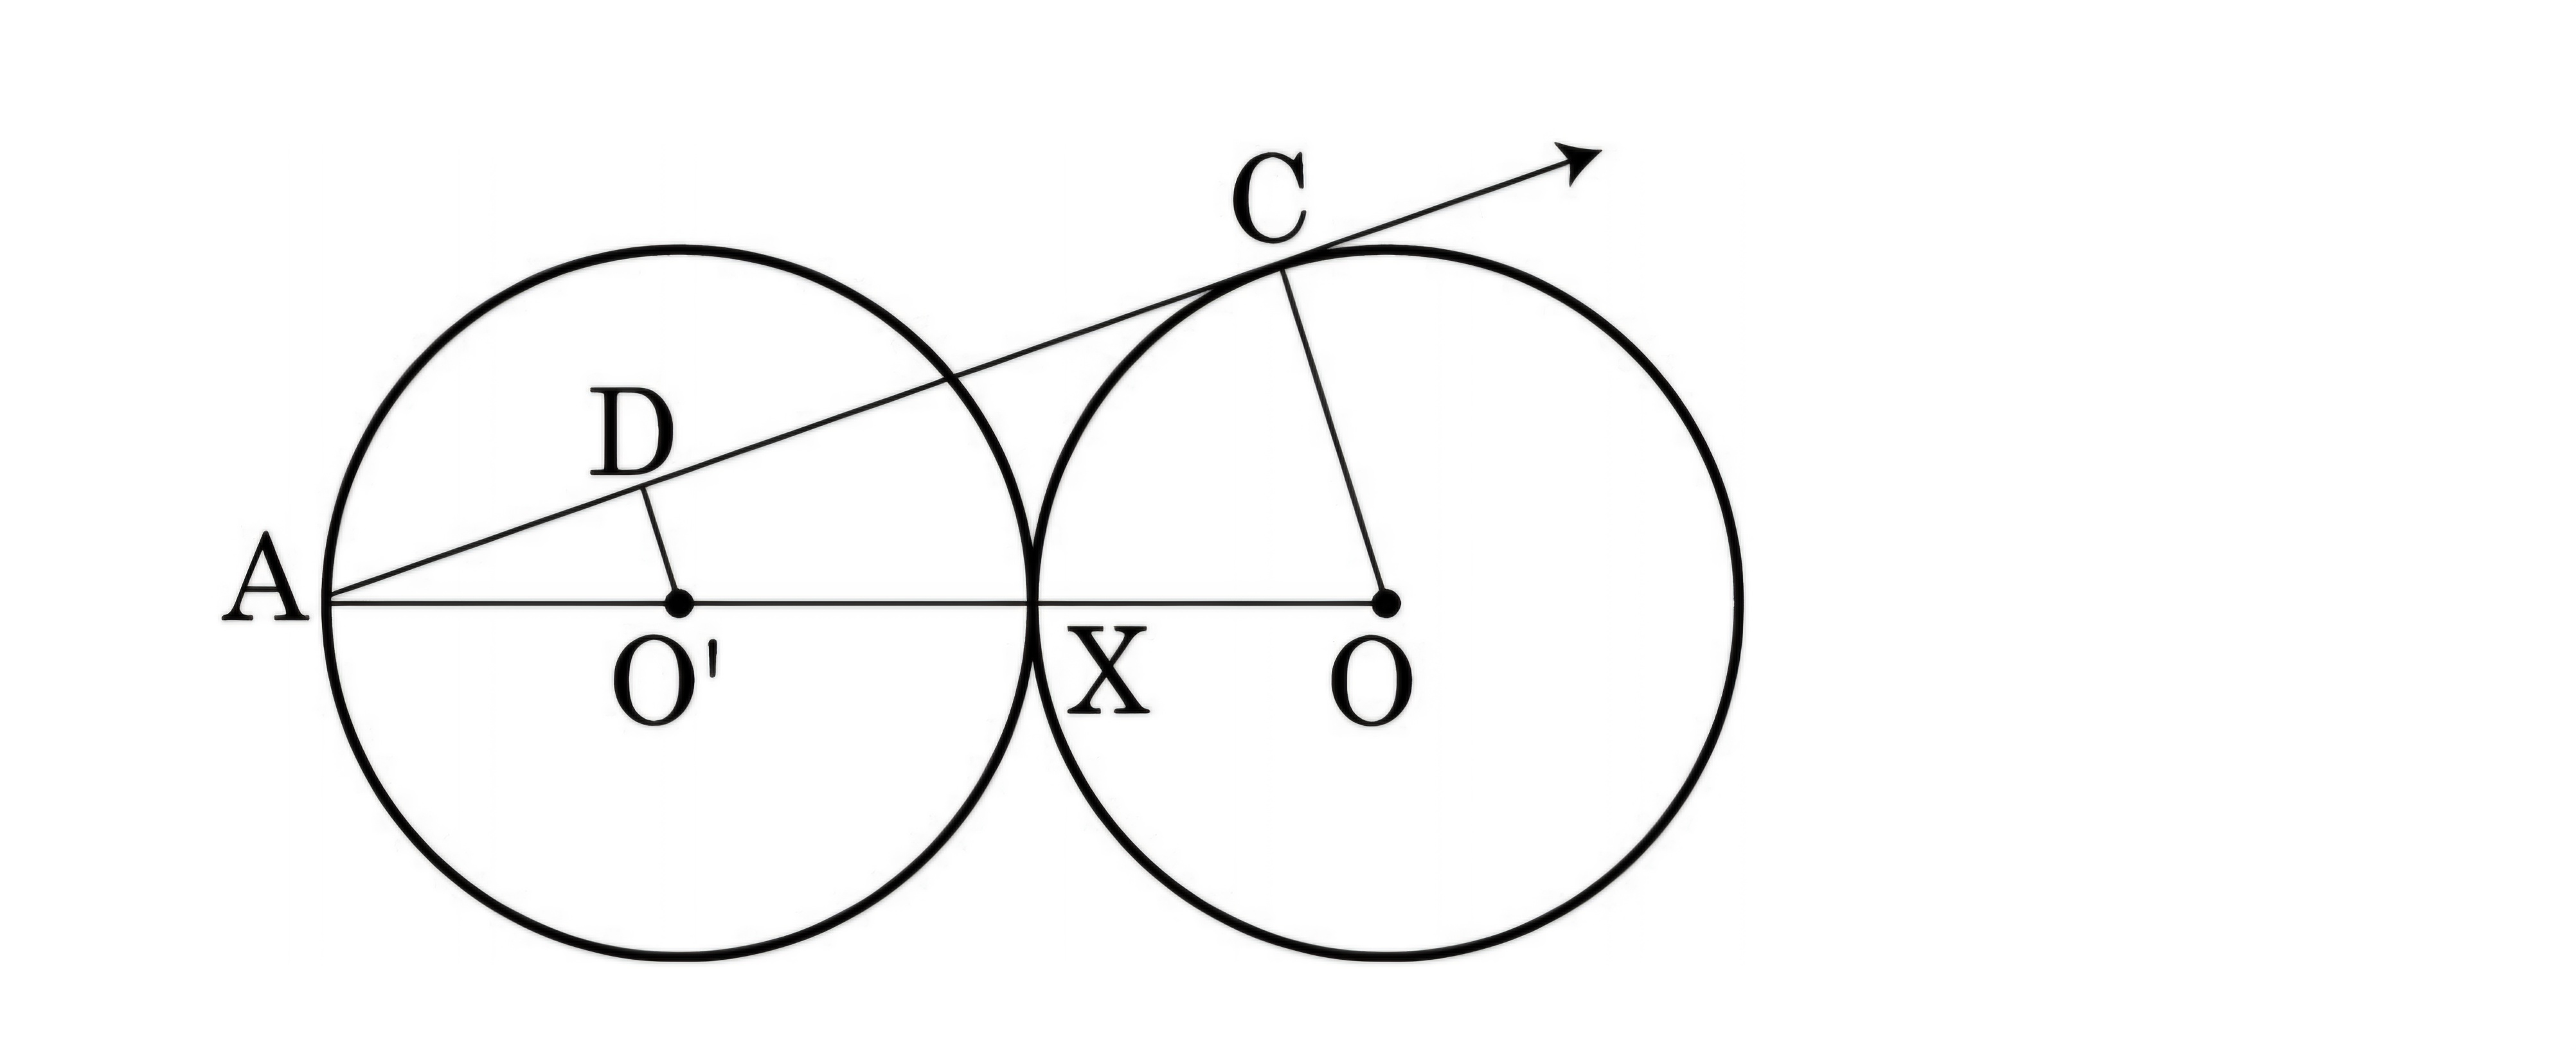
\includegraphics[width=\columnwidth]{./figs/twocircle.jpg}
    \caption{Two equal circles}
     \label{fig:twocircle}
     \end{figure}
\item solve for $x$ :
	\begin{align}
		\frac{1}{x+1}+\frac{2}{x+2}=\frac{4}{x+4},x \not=-1,-2,-4
	\end{align}
\item the angle of elevation of the $Q$ of a vertical tower $PQ$ from a point $X$ n the ground is $60^{\degree}$. From $Y,40 m$ vertically above $X$ the angle of elevation of the top $Q$ of tower is $45^{\degree}$. Find the height of the tower $PQ$ and the distance $PX$ (use $\sqrt{3}=1.73$)	
\item A number $x$ is selected at random from the numbers $1,2,3$ and $4$.Another number $y$ is selected at random from the numbrs $1,4,9$ and $16$. Find the probability that product of $x$ and $y$ is less than $16$.
\end{enumerate}
\end{document}	
